% Generated 2021-01-06 15:42:26 +0530
\subsection{Relationships} \label{sec:Relationships}


\begin{figure}[ht]
  \centering
    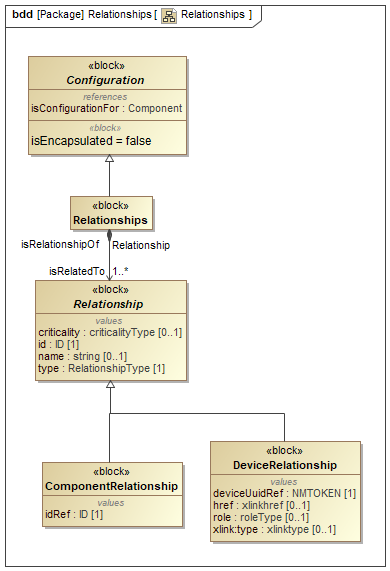
\includegraphics[width=1.0\textwidth]{figures/Relationships.png}
  \caption{Relationships Diagram}
  \label{fig:Relationships}
\end{figure}

\FloatBarrier



\subsubsection{Relationship}
\label{sec:Relationship}



\block{Relationship} describes the association between two pieces of equipment that function independently but together perform a manufacturing operation.


\paragraph{Attributes of Relationship}\mbox{}
\label{sec:Attributes of Relationship}

\tbl{Attributes of Relationship} lists the attributes of \texttt{Relationship}.

\begin{table}[ht]
\centering 
  \caption{Attributes of Relationship}
  \label{table:Attributes of Relationship}
\tabulinesep=3pt
\begin{tabu} to 6in {|l|l|l|} \everyrow{\hline}
\hline
\rowfont\bfseries {Attribute} & {Type} & {Multiplicity} \\
\tabucline[1.5pt]{}

\property{name}[Relationship] & \texttt{string} & 0..1 \\
\end{tabu}
\end{table}
\FloatBarrier

Descriptions for attributes of \block{Relationship}:

\begin{itemize}

\item \property{name}[Relationship] \newline The name associated with this \block{Relationship}.
\end{itemize}

\subsubsection{ComponentRelationship}
\label{sec:ComponentRelationship}



\block{ComponentRelationship} describes the association between two components within a piece of equipment that function independently but together perform a capability or service within a piece of equipment.


\paragraph{Attributes of ComponentRelationship}\mbox{}
\label{sec:Attributes of ComponentRelationship}

\tbl{Attributes of ComponentRelationship} lists the attributes of \texttt{ComponentRelationship}.

\begin{table}[ht]
\centering 
  \caption{Attributes of ComponentRelationship}
  \label{table:Attributes of ComponentRelationship}
\tabulinesep=3pt
\begin{tabu} to 6in {|l|l|l|} \everyrow{\hline}
\hline
\rowfont\bfseries {Attribute} & {Type} & {Multiplicity} \\
\tabucline[1.5pt]{}

\property{idRef}[ComponentRelationship] & \texttt{ID} & 1 \\
\property{criticality}[ComponentRelationship] & \texttt{criticalityType} & 0..1 \\
\property{id}[ComponentRelationship] & \texttt{ID} & 1 \\
\property{type}[ComponentRelationship] & \texttt{RelationshipType} & 1 \\
\end{tabu}
\end{table}
\FloatBarrier

Descriptions for attributes of \block{ComponentRelationship}:

\begin{itemize}

\item \property{idRef}[ComponentRelationship] \newline A reference to the associated component element.

\item \property{criticality}[ComponentRelationship] \newline Defines whether the services or functions provided by the associated piece of equipment is required for the operation of this piece of equipment.

\texttt{criticalityType} Enumeration:

\begin{itemize}
\item \texttt{CRITICAL} \newline The services or functions provided by the associated element is required for the operation of this element. 
\item \texttt{NONCRITICAL} \newline The services or functions provided by the associated element is not required for the operation of this element. 
\end{itemize}


\item \property{id}[ComponentRelationship] \newline The unique identifier for this \block{Relationship}.

\item \property{type}[ComponentRelationship] \newline Defines the authority that this piece of equipment has relative to the associated piece of equipment.

\texttt{RelationshipType} Enumeration:

\begin{itemize}
\item \texttt{PARENT} \newline This element functions as a parent in the relationship with the associated element. 
\item \texttt{CHILD} \newline This element functions as a child in the relationship with the associated element. 
\item \texttt{PEER} \newline This element functions as a peer which provides equal functionality and capabilities in the relationship with the associated element. 
\end{itemize}

\end{itemize}

\subsubsection{DeviceRelationship}
\label{sec:DeviceRelationship}



\block{DeviceRelationship} describes the association between two pieces of equipment that function independently but together perform a manufacturing operation.


\paragraph{Attributes of DeviceRelationship}\mbox{}
\label{sec:Attributes of DeviceRelationship}

\tbl{Attributes of DeviceRelationship} lists the attributes of \texttt{DeviceRelationship}.

\begin{table}[ht]
\centering 
  \caption{Attributes of DeviceRelationship}
  \label{table:Attributes of DeviceRelationship}
\tabulinesep=3pt
\begin{tabu} to 6in {|l|l|l|} \everyrow{\hline}
\hline
\rowfont\bfseries {Attribute} & {Type} & {Multiplicity} \\
\tabucline[1.5pt]{}

\property{deviceUuidRef}[DeviceRelationship] & \texttt{NMTOKEN} & 1 \\
\property{href}[DeviceRelationship] & \texttt{xlinkhref} & 0..1 \\
\property{role}[DeviceRelationship] & \texttt{roleType} & 0..1 \\
\property{xlink:type}[DeviceRelationship] & \texttt{xlinktype} & 0..1 \\
\property{criticality}[DeviceRelationship] & \texttt{criticalityType} & 0..1 \\
\property{id}[DeviceRelationship] & \texttt{ID} & 1 \\
\property{type}[DeviceRelationship] & \texttt{RelationshipType} & 1 \\
\end{tabu}
\end{table}
\FloatBarrier

Descriptions for attributes of \block{DeviceRelationship}:

\begin{itemize}

\item \property{deviceUuidRef}[DeviceRelationship] \newline A reference to the associated piece of equipment. 


\item \property{href}[DeviceRelationship] \newline A URI identifying the \gls{Agent} that is publishing information for the associated piece of equipment. \property{href} \textbf{MUST} also include the UUID for that specific piece of equipment.

\property{href} is of type \texttt{xlink:href} from the W3C XLink specification: \textit{https://www.w3.org/TR/xlink11/}.

\item \property{role}[DeviceRelationship] \newline Defines the services or capabilities that the referenced piece of equipment provides relative to this piece of equipment.

\texttt{roleType} Enumeration:

\begin{itemize}
\item \texttt{SYSTEM} \newline The associated element performs the functions of a \block{System} for this element. 
\item \texttt{AUXILIARY} \newline The associated element performs the functions as an \texttt{Auxiliary} for this element. 
\end{itemize}


\item \property{xlink:type}[DeviceRelationship] \newline The XLink \property{type} attribute \textbf{MUST} have a fixed value of \texttt{locator} as defined in W3C XLink 1.1 \textit{https://www.w3.org/TR/xlink11/}.

If the \property{href} attribute is provided, it \textbf{MUST} conform to the URI syntactic rules as defined in IETF RFC 3986 for Uniform Resource Identifiers. \textit{https://www.ietf.org/rfc/rfc3986.txt}

\item \property{criticality}[DeviceRelationship] \newline Defines whether the services or functions provided by the associated piece of equipment is required for the operation of this piece of equipment.

\item \property{id}[DeviceRelationship] \newline The unique identifier for this \block{Relationship}.

\item \property{type}[DeviceRelationship] \newline Defines the authority that this piece of equipment has relative to the associated piece of equipment.
\end{itemize}

\subsubsection{Relationships}
\label{sec:Relationships}



\block{Relationships} \glspl{organize} \block{Relationship} elements.


\paragraph{Elements of Relationships}\mbox{}
\label{sec:Elements of Relationships}

\tbl{Elements of Relationships} lists the elements of \texttt{Relationships}.

\begin{table}[ht]
\centering 
  \caption{Elements of Relationships}
  \label{table:Elements of Relationships}
\tabulinesep=3pt
\begin{tabu} to 6in {|l|l|} \everyrow{\hline}
\hline
\rowfont\bfseries {Element} & {Multiplicity} \\
\tabucline[1.5pt]{}
\texttt{Relationship} & 1..* \\
\end{tabu}
\end{table}
\FloatBarrier


Descriptions for elements of \block{Relationships}:

\begin{itemize}

\item \block{Relationship} \newline \block{Relationship} describes the association between two pieces of equipment that function independently but together perform a manufacturing operation.
\end{itemize}
